% This voodoo is needed for arXiv scripts and must appear within the first 4 lines
\pdfoutput=1
\documentclass[aps,prd,amsmath,floats,floatfix, twocolumn,
superscriptaddress,nofootinbib,showpacs]{revtex4-1}

% UTF8 always
\usepackage[T1]{fontenc}
\usepackage[utf8]{inputenc}
\usepackage{lmodern}

\usepackage{verbatim}

\usepackage[dvipsnames, usenames]{xcolor}
\definecolor{linkcolor}{rgb}{0.0,0.3,0.5}
\usepackage[hypertexnames=false, unicode, colorlinks=true, linkcolor=linkcolor,
citecolor=linkcolor, filecolor=linkcolor,urlcolor=linkcolor,
pdfusetitle]{hyperref}

%\usepackage[colorlinks, pdfborder={0 0 0}, plainpages=false]{hyperref}
\usepackage[all]{hypcap}
\usepackage{graphicx}
\usepackage{xspace}
%\usepackage[usenames,dvipsnames]{color}
\usepackage{amssymb}
\usepackage[normalem]{ulem} %for \sout
\usepackage{bm} % boldmath

% Better spacing
\usepackage{microtype}

\usepackage[english]{babel}
\usepackage{blindtext}

%
\graphicspath{%
  {figs/}%
  % More directories are added in braces, without commas between
}


\DeclareMathAlphabet{\mathpzc}{OT1}{pzc}{m}{it}

\newcommand{\roughly}{\mathchar"5218\relax\,} % Different from \sim in spacing
\newcommand{\into}{\!\times\!\relax} % Different from \times in spacing

% Macros for text changes
\newcommand{\red}{\textcolor{red}}
\newcommand{\vv}[1]{\textcolor{WildStrawberry}{VV: #1}}

\newcommand{\Note}[1]{\textcolor{blue}{\textbf{[#1]}}}
\newcommand{\h}{\mathpzc{h}}
\newcommand{\hlm}{\mathpzc{h}_{\ell m}}
\newcommand{\chieff}{\chi_{\mathrm{eff}}}
\newcommand{\chiPN}{\chi_{\mathrm{PN}}}


\newcommand{\bfemph}[1]{\emph{\textbf{#1}}}

\newcommand{\nn}{\nonumber}

\newcommand{\cd}{\nabla}
\newcommand{\pd}{\partial}
\newcommand{\lie}{\mathcal{L}}
\newcommand{\dd}{\mathrm{d}}

\newcommand{\TODO}[1]{\red{TODO: #1}}
\newcommand{\AddCite}{\red{[Needs citation]}}


% \newcommand{\mat}{{\tiny{\mathrm{mat}}}}
% \newcommand{\mat}{{(\mathrm{m})}}
\newcommand{\txt}[1]{{\textrm{\tiny{#1}}}}

%%%%%%%%%%%%%%%%%%%%%%%%%%%%%%%%%%%%%%%%%%%%%%%%%%%%%%%%%%%%%%%%%%%%%%%%%%%
\begin{document}

\title{The greatest science}

\newcommand{\Cornell}{\affiliation{Cornell Center for Astrophysics
    and Planetary Science, Cornell University, Ithaca, New York 14853, USA}}
\newcommand\CornellPhys{\affiliation{Department of Physics, Cornell
    University, Ithaca, New York 14853, USA}}
\newcommand\Caltech{\affiliation{TAPIR 350-17, California Institute of
    Technology, 1200 E California Boulevard, Pasadena, CA 91125, USA}}
\newcommand{\AEI}{\affiliation{Max Planck Institute for Gravitational Physics
    (Albert Einstein Institute), Am M\"uhlenberg 1, Potsdam 14476, Germany}} %
\newcommand{\UMassD}{\affiliation{Department of Mathematics,
    Center for Scientific Computing and Visualization Research,
    University of Massachusetts, Dartmouth, MA 02747, USA}}
\newcommand\Olemiss{\affiliation{Department of Physics and Astronomy,
    The University of Mississippi, University, MS 38677, USA}}
\newcommand{\Bham}{\affiliation{School of Physics and Astronomy and Institute
    for Gravitational Wave Astronomy, University of Birmingham, Birmingham, B15
    2TT, UK}}
\newcommand{\ICTS}{\affiliation{International Centre for Theoretical Sciences,
    Tata Institute of Fundamental Research, Bangalore 560089, India}}

\author{Md Arif Shaikh}
\email{arif.shaikh@icts.res.in}
\ICTS
\author{Vijay Varma}
\email{vijay.varma@aei.mpg.de}
\thanks{Marie Curie Fellow}
\AEI

% Because hyperref only gets the *last* author, we need to be explicit.
\hypersetup{pdfauthor={Varma et al.}}

\date{\today}

%==========================================================================
\begin{abstract}
Eccentric CBCs are important science targets of GW observatories. Many different eccentricity definitions exist in the literature.
This paper continues the development of a definition of eccentricity that is defined based solely on the gauge invariant gravitational
waveforms and applicable to gravitational waveforms of many origins. Our proposal improves on related works in that the new definition
agrees in the Newtonian limit with the standard Newtonian definition of eccentricity. We present a public implementation of the
proposed algorithm and demonstrate its robustness on waveforms of various origin, ranging from quasi-circular to highly eccentric systems.
The present work focuses on aligned-spin binaries which do not exhibit orbital precession. Possible extensions to precessing binaries are discussed.
\end{abstract}

\maketitle

%==========================================================================
\section{Introduction}
\label{sec:introduction}
I done did it. Some other people that done'd similar things:
\cite{Scott:2015rza}.

%==========================================================================
\section{Methods}
\label{sec:methods}
Here's how I done'd it.

%--------------------------------------------------------------------------
\begin{figure}[thb]
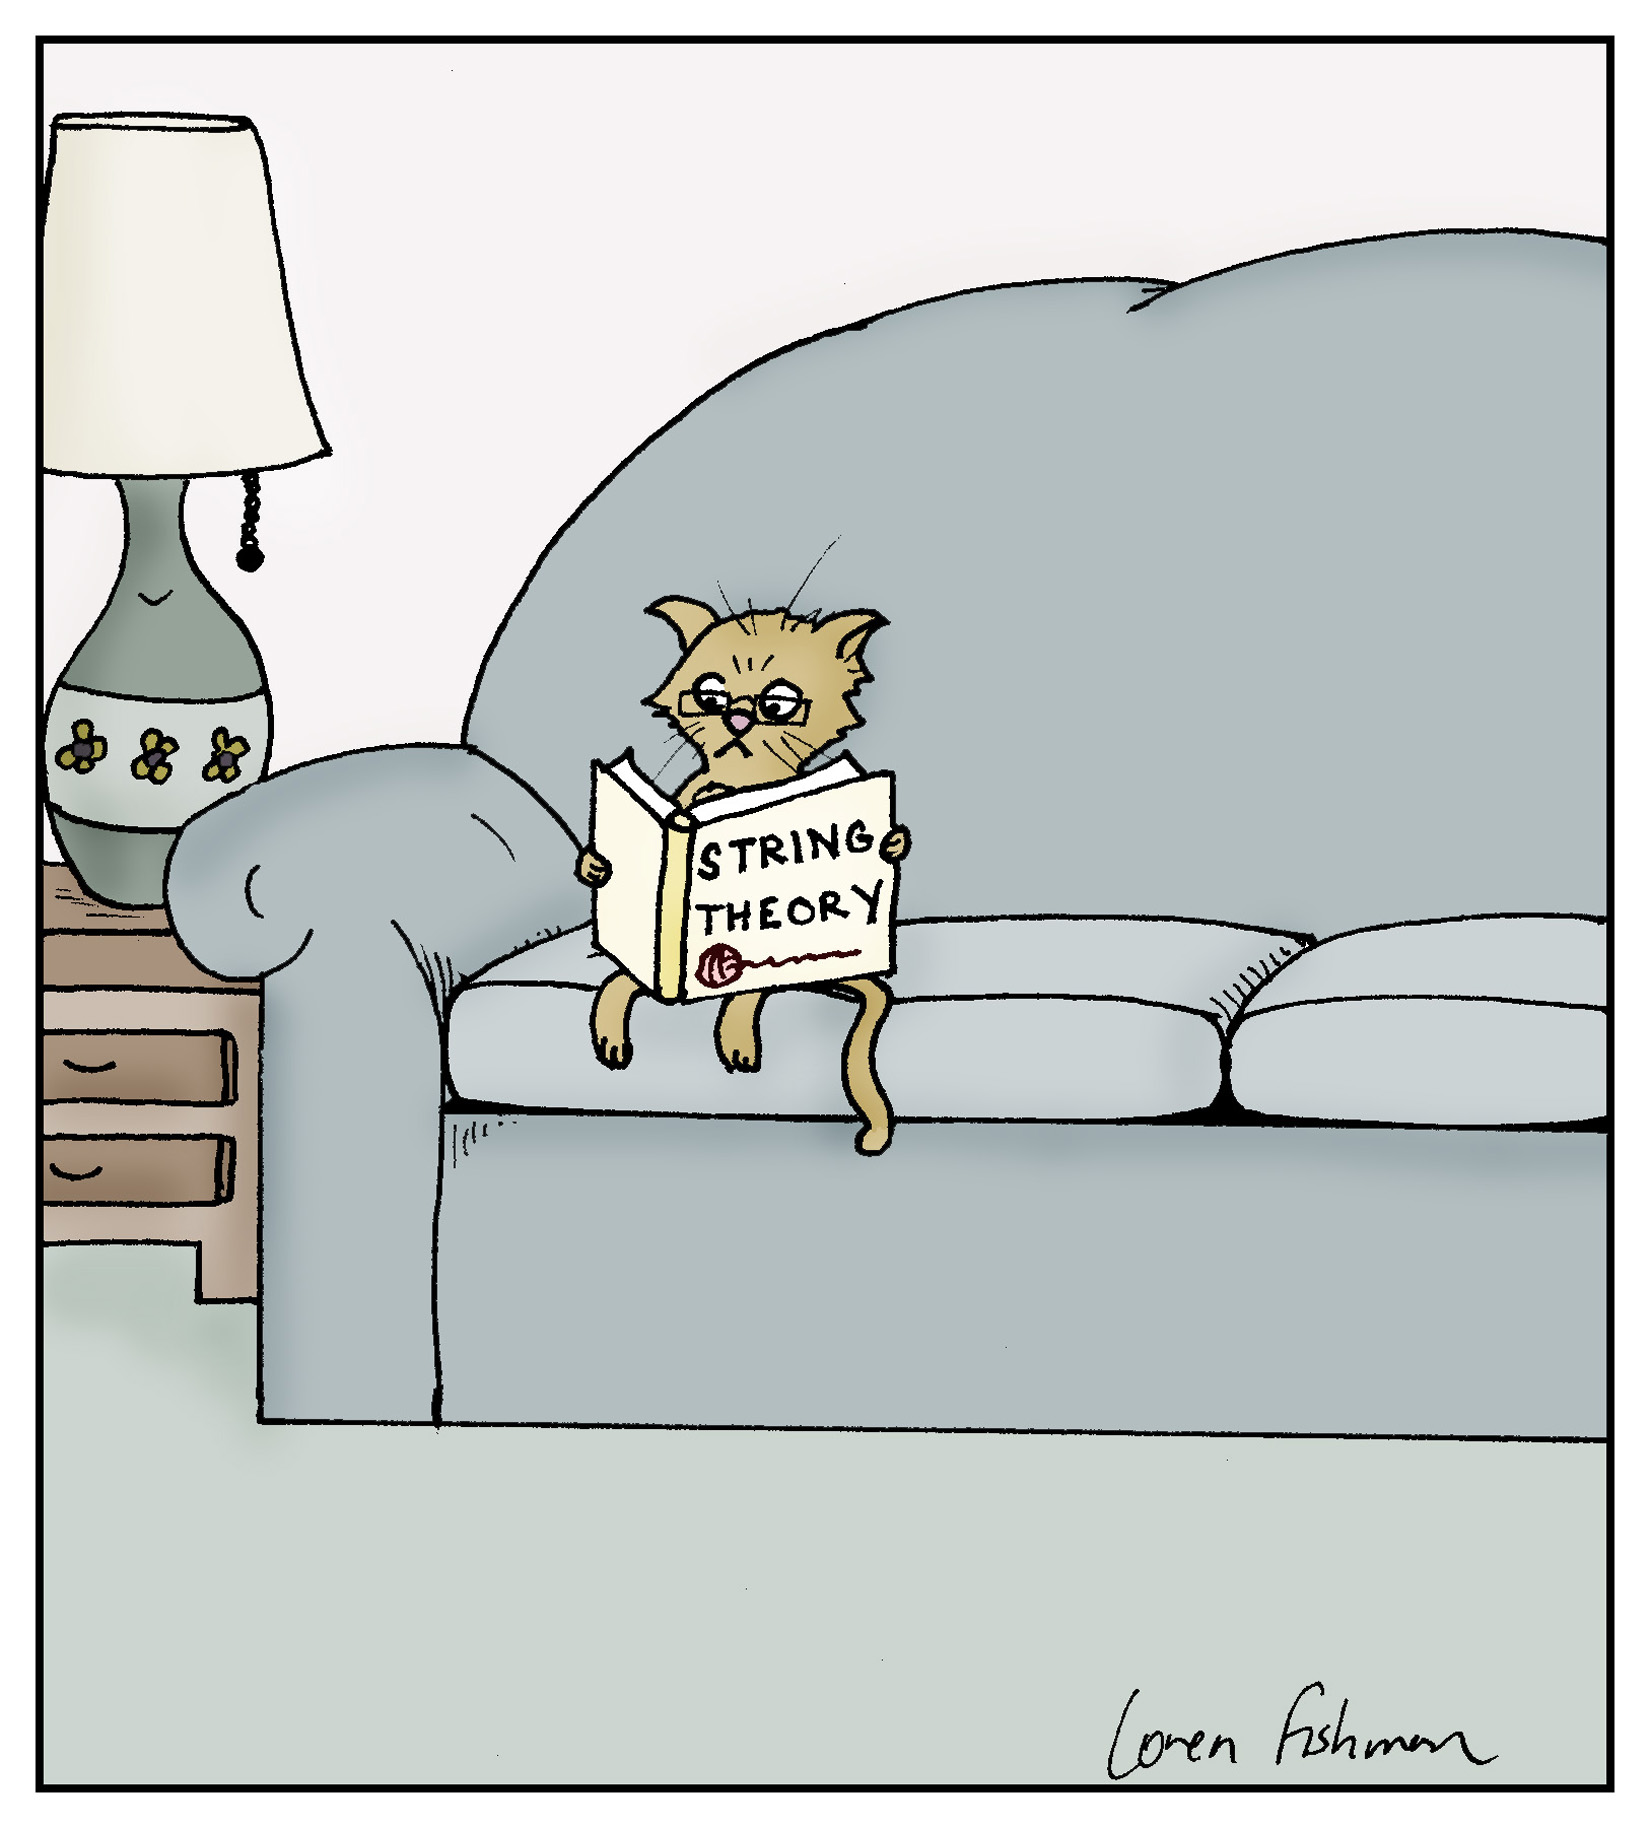
\includegraphics[width=0.45\textwidth]{string_cat.jpeg}
\caption{
What happened to Schrodinger's cat?
}
\label{fig:strings}
\end{figure}

%==========================================================================
\section{Results}
\label{sec:results}
Here's what I found after I done'd it.

And Maxwell said:
\begin{gather}
    dF = 0, \\
    d_{\star}F = \mu_0 \, J.
\label{eq:doppler_mass}
\end{gather}
and then there was light.


%==========================================================================
\section{Conclusion}
\label{sec:conclusion}
Here's what you should learn now that I done'd it.


%==========================================================================
\begin{acknowledgments}
% Randos
We thank Bob Loblaw for useful discussions.
% VV
V.V acknowledges support from the European Union’s Horizon 2020 research and
innovation program under the Marie Skłodowska-Curie grant agreement No.~896869.
% LIGO
This material is based upon work supported by NSF's LIGO Laboratory which is a
major facility fully funded by the NSF.
% GWOSC
%This research made use of data, software and/or web tools obtained from the
%Gravitational Wave Open Science Center~\cite{GW_open_science_center}, a service
%of the LIGO Laboratory, the LIGO Scientific Collaboration and the Virgo
%Collaboration.
\end{acknowledgments}

%%%%%%%%%%%%%%%%%%%%%%%%%%%%%%%%%%%%%%%%%%%%%%%%%%%%%%%%%%%%%%%%%%%%%%%%%%%%%%%
\section*{References}
%%%%%%%%%%%%%%%%%%%%%%%%%%%%%%%%%%%%%%%%%%%%%%%%%%%%%%%%%%%%%%%%%%%%%%%%%%%%%%%
\bibliography{References}


\end{document}
